\subsection{Function Call by RPR}

OlaVM adopts the register-based model. In order to easier simulate the effect of a function call stack it is necessary to save the next \verb|pc| that currently calls the initiating function to a dedicated read-only memory, RPR (Return PC ROM), which is convenient to find the \verb|pc| position that the last call should return to after the execution of the sub-function. The function call involves two instructions, \verb|CALL| and \verb|RET|, and a special register \verb|fp|, which points to the address of RPR. Figure \ref{fig:function-call-example} shows a function call example.
\begin{figure}[!ht]
    \centering
    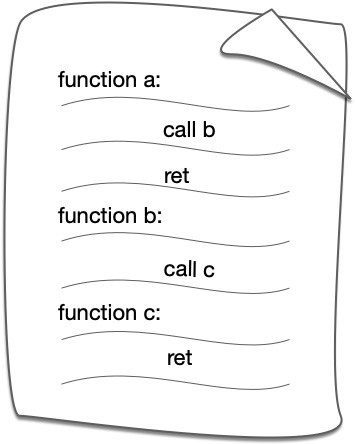
\includegraphics[width=0.3\textwidth]{function-call-example.jpg}
    \caption{Function call example}
    \label{fig:function-call-example}
\end{figure}

The stack frame of the above function call is shown in Figure \ref{fig:function-call-frame}.
\begin{figure}[!ht]
    \centering
    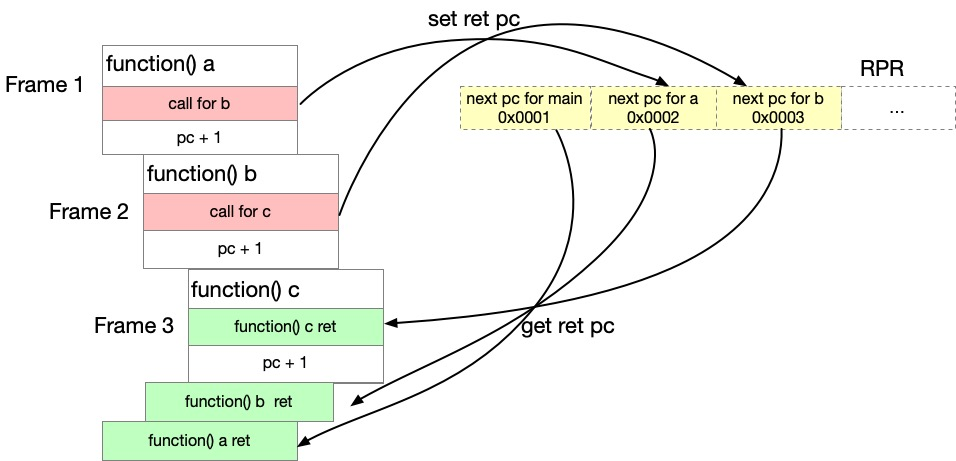
\includegraphics[width=0.8\textwidth]{function-call-frame.jpg}
    \caption{Function call frame}
    \label{fig:function-call-frame}
\end{figure}

\begin{itemize}
    \item RPR stores 3 return \verb|pc| positions: \verb|a return -> main pc|, \verb|b return -> a pc|, \verb|c return -> b pc|;
    \item When function \verb|main| utilizes instruction \verb|CALL| to call function \verb|a|, the value of \verb|pc| will be updated to the value saved in register \verb|r0|;
    \item Set the value of ROM location pointed by the pointer stored in register \verb|fp| to current \verb|pc+1|, \verb|fp+1| points to the next empty memory area.
    \item When the function a completes the execution, it will take the value pointing to the correct position of ROM through the pointer stored in register \verb|fp|. Set current \verb|pc| to this value, so the remaining program fragments can be executed when returning to function main;
    \item \verb|fp| points to the position of \verb|fp-1| in RPR;
    \item For nested calls of function \verb|b| and function \verb|c|, the change process of \verb|pc| and \verb|fp| is the same as above.
\end{itemize}
